\documentclass[10pt,a4paper]{report}
%\usepackage[latin1]{inputenc}
\usepackage[utf8]{inputenc}
\usepackage{amsmath}
\usepackage{amsfonts}
\usepackage{amssymb}
\usepackage{graphicx}
\usepackage{multicol}
\usepackage{tabularx}
\usepackage{tikz}
\usetikzlibrary{arrows,shapes,automata,petri,positioning,calc}
\usepackage{hyperref}
\usepackage{tikz}
\usetikzlibrary{matrix,calc}
\usepackage[margin=0.5in]{geometry}
\newenvironment{Figure}
  {\par\medskip\noindent\minipage{\linewidth}}
  {\endminipage\par\medskip}
\begin{document}
%--------------------logo figure-------------------------%
\begin{figure*}[!tbp]
  \centering
  \begin{minipage}[b]{0.4\textwidth}
    
\includegraphics[scale = 0.05]{iitlogo.jpg}
  \end{minipage}
  \hfill
  \vspace{5mm}\begin{minipage}[b]{0.4\textwidth}
\raggedleft  
\includegraphics[scale = 0.10]{nrc.png}\

  \end{minipage}\vspace{0.2cm}
\end{figure*}
%--------------------name & rollno-----------------------
\raggedright \textbf{Name}:\hspace{1mm} Chirag Shah\hspace{3cm} \Large \textbf{ASSIGNMENT-2}\hspace{2.5cm} % 
\normalsize \textbf{Roll No.} :\hspace{1mm} FWC22053\vspace{1mm}
\begin{center}
\textbf{Using assembly language}\hspace{1cm}   \vspace{1cm}
\end{center}
\begin{multicols}{2}


%-----------------Sequence Detector-----------------------------%
\textbf{Sequence Detector}
\vspace{0.5cm}\raggedright \\A sequence detector is a sequential state machine that takes an input string of bits and generates an output 1 whenever the target sequence has been detected. In a Mealy machine, output depends on the present state and the external input (x).\vspace{3mm} \\ 
%------------------------working-------------------%
\textbf{Working}\vspace{1mm}
\raggedright \\A sequence detector accepts as input a string of bits: either 0 or 1. Its output goes to 1 when a target sequence has been detected.\vspace{3mm} \\ 
\raggedright There are two basic types:\vspace{3mm} 
\begin{itemize}
\item Overlap
\item Non-overlap. \vspace{2mm}
\end{itemize}
%----------------problem statement--------------%
\raggedright \textbf{Problem Statement:}\vspace{2mm}
\raggedright \\Using Platformio CLI wite a programm to identify if the Sequence is either  11 or 00110 .

\vspace{5mm}

%-----------------------------solution---------------------------
\raggedright \textbf{SOLUTION}:\vspace{2mm}
\raggedright Steps for using State Diagram:
\\1.To detect 00110 and 11 . first input is given to SO . if the first bit i/p is 0 it will go to next state i.e S1 and o/p will be 0 (LED=OFF) . 
\\2.If the i/p is 1 it will go to state S5. o/p will be 0 (LED=OFF)
\\3.Same steps will be repeated for all states  .
\\4.when it detects 00110 the o/p will be 1 (LED=ON)
\\5.Same as above if it detects 11 o/p will be 1 (LED=ON)
\\6.Again it repeats as it is overlapping. \\

%--------------------state diagram------------------------------%

\vspace{1cm}
\textbf{State Diagram}
\vspace{0.4cm}
\usetikzlibrary{arrows,shapes,automata,petri,positioning,calc}

\tikzset{
    place/.style={
        circle,
        thick,
        draw=black,
        fill=gray!50,
        minimum size=6mm,
    },
        state/.style={
        circle,
        thick,
        draw=blue!75,
        fill=blue!20,
        minimum size=6mm,
    },
}

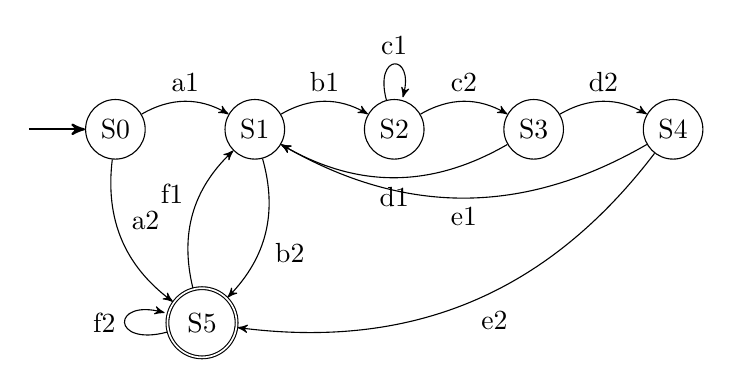
\begin{tikzpicture}[node distance=2cm and 1cm,>=stealth',auto, every place/.style={draw}]
    \node [place] (S0) {S0};
    \coordinate[node distance=1.1cm,left of=S0] (left-S0);
    \coordinate[node distance=1.1cm,right of=S0] (right-S0);

    \draw[->, thick] (left-S0) -- (S0);

    \node [place] (S1) [right=of S0] {S1};
    \node [place] (S2) [right=of S1] {S2};
    \node [place] (S3) [right=of S2] {S3};
    \node [place] (S4) [right=of S3] {S4};
    \node [state,initial text=,accepting by double] (S5) [below =of right-S0] {S5};

    


    \path[->] (S0) edge [bend left] node {a1}(S1);
    \path[->] (S0) edge [bend right] node {a2} (S5);
    
    \path[->] (S1) edge [bend left] node {b1} (S2);
    \path[->] (S1) edge [bend left] node {b2} (S5);
    
    \path[->] (S2) edge [loop above] node {c1} (S2);
    \path[->] (S2) edge [bend left] node {c2} (S3);
    
    \path[->] (S3) edge [bend left] node {d1} (S1);  
    \path[->] (S3) edge [bend left] node {d2} (S4);  
    
    \path[->] (S4) edge [bend left] node {e1} (S1);  
    \path[->] (S4) edge [bend left] node {e2} (S5);  
    
    \path[->] (S5) edge [bend left] node {f1} (S1);  
    \path[->] (S5) edge [loop left] node {f2} (S5);  

\end{tikzpicture}
\vspace{1.5cm}
%-------------------State Diagrams-------------%

\textbf{State Diagram -Input and Outputs}

  \setlength{\arrayrulewidth}{0.5mm} \begin{center}
      

  \setlength{\tabcolsep}{6.9pt}
  \renewcommand{\arraystretch}{2.2}
  \begin{tabular}{|l|c|c|l|c|}
  \hline 
  \textbf{values} & \textbf{Input} & \textbf{output} & \textbf{states} &\textbf{Next state} \\
  \hline \hline
    a1 & 0 & 0 & S0 & S1 \\ \hline
    a2 & 1 & 0 & S0 & S5\\  \hline \hline
    b1 & 0 & 0 & S1 & S2\\ \hline
    b2 & 1 & 0 & S1 & S5\\ \hline \hline
    c1 & 0 & 0 & S2 & S2\\ \hline
    c2 & 1 & 0 & S2 & S3\\ \hline \hline
    d1 & 0 & 0 & S3 & S1\\ \hline
    d2 & 1 & 0 & S3 & S4\\ \hline \hline
    e1 & 0 & 1 & S4 & S1\\ \hline
    e2 & 1 & 0 & S4 & S5\\ \hline\hline
    f1 & 0 & 0 & S5 & S1\\ \hline
    f2 & 1 & 1 & S5 & S5\\ 
    \hline 
      \end{tabular}
  \end{center} \vspace{2mm}
  \vspace{0.5cm}
\textbf{Components}
 \begin{center} \setlength{\arrayrulewidth}{0.5mm} 
  \setlength{\tabcolsep}{15pt}
  \renewcommand{\arraystretch}{1.3}
  \begin{tabular}{|l|c|c|}
  \hline 
  \textbf{Component} & \textbf{Value} & \textbf{Quantity} \\
  \hline \hline
    Breadboard & - & 1\\ \hline
    Resistor & 220 ohms & 1\\ \hline
    Arduino & Uno & 1\\ \hline
    Led & 5v & 1\\ \hline
    Flip Flop & 7474 & 2\\ \hline
    Jumper Wires & - & 20\\ 
   
    \hline
      \end{tabular}
  \end{center}
  \textbf{Truth table}
  \begin{center}
    \label{tab:truthtable}
    \setlength{\arrayrulewidth}{0.5mm}
\setlength{\tabcolsep}{9.9pt}
\renewcommand{\arraystretch}{1.5}
    \begin{tabular}{|l|c|r|l|c|l|c|l|}
    \hline % <-- Alignments: 1st column left, 2nd middle and 3rd right, with vertical lines in between
      \textbf{q2} & \textbf{q1} & \textbf{q0} & \textbf{x} & \textbf{d2} & \textbf{d1} & \textbf{d0} & \textbf{y}\\
      \hline  \hline
      0 & 0 & 0 & 0 & 0 & 0 & 1 & 0\\  \hline
      0 & 0 & 0 & 1 & 1 & 0 & 1 & 0\\  \hline
      0 & 0 & 1 & 0 & 0 & 1 & 0 & 0\\  \hline
      0 & 0 & 1 & 1 & 1 & 0 & 1 & 0\\ \hline
      0 & 1 & 0 & 0 & 0 & 1 & 0 & 0\\ \hline
      0 & 1 & 0 & 1 & 0 & 1 & 1 & 0\\  \hline
      0 & 1 & 1 & 0 & 0 & 0 & 1 & 0\\ \hline
      0 & 1 & 1 & 1 & 1 & 0 & 0 & 0\\ \hline
      1 & 0 & 0 & 0 & 0 & 0 & 1 & 1\\ \hline
      1 & 0 & 0 & 1 & 1 & 0 & 1 & 0\\ \hline
      1 & 0 & 1 & 0 & 0 & 0 & 1 & 0\\ \hline
      1 & 0 & 1 & 1 & 1 & 0 & 1 & 1\\ \hline
      1 & 1 & 0 & 0 & x & x & x & x\\ \hline
      1 & 1 & 0 & 1 & x & x & x & x\\ \hline
      1 & 1 & 1 & 0 & x & x & x & x\\ \hline
      1 & 1 & 1 & 1 & x & x & x & x\\ \hline
      1 & 1 & 1 & 1 & x & x & x & x\\ 
      \hline
    \end{tabular}
  \end{center} \vspace{2.5mm}
 %-----------------kmap-----------------
 %isolated term
%#1 - Optional. Space between node and grouping line. Default=0
%#2 - node
%#3 - filling color

\newcommand{\implicantsol}[3][0]{
    \draw[rounded corners=3pt, fill=#3, opacity=0.3] ($(#2.north west)+(135:#1)$) rectangle ($(#2.south east)+(-45:#1)$);
    }


%internal group
%#1 - Optional. Space between node and grouping line. Default=0
%#2 - top left node
%#3 - bottom right node
%#4 - filling color
\newcommand{\implicant}[4][0]{
    \draw[rounded corners=3pt, fill=#4, opacity=0.3] ($(#2.north west)+(135:#1)$) rectangle ($(#3.south east)+(-45:#1)$);
    }

%group lateral borders
%#1 - Optional. Space between node and grouping line. Default=0
%#2 - top left node
%#3 - bottom right node
%#4 - filling color
\newcommand{\implicantcostats}[4][0]{
    \draw[rounded corners=3pt, fill=#4, opacity=0.3] ($(rf.east |- #2.north)+(90:#1)$)-| ($(#2.east)+(0:#1)$) |- ($(rf.east |- #3.south)+(-90:#1)$);
    \draw[rounded corners=3pt, fill=#4, opacity=0.3] ($(cf.west |- #2.north)+(90:#1)$) -| ($(#3.west)+(180:#1)$) |- ($(cf.west |- #3.south)+(-90:#1)$);
}

%group top-bottom borders
%#1 - Optional. Space between node and grouping line. Default=0
%#2 - top left node
%#3 - bottom right node
%#4 - filling color
\newcommand{\implicantdaltbaix}[4][0]{
    \draw[rounded corners=3pt, fill=#4, opacity=0.3] ($(cf.south -| #2.west)+(180:#1)$) |- ($(#2.south)+(-90:#1)$) -| ($(cf.south -| #3.east)+(0:#1)$);
    \draw[rounded corners=3pt, fill=#4, opacity=0.3] ($(rf.north -| #2.west)+(180:#1)$) |- ($(#3.north)+(90:#1)$) -| ($(rf.north -| #3.east)+(0:#1)$);
}

%group corners
%#1 - Optional. Space between node and grouping line. Default=0
%#2 - filling color
\newcommand{\implicantcantons}[2][0]{
    \draw[rounded corners=3pt, opacity=.3] ($(rf.east |- 0.south)+(-90:#1)$) -| ($(0.east |- cf.south)+(0:#1)$);
    \draw[rounded corners=3pt, opacity=.3] ($(rf.east |- 8.north)+(90:#1)$) -| ($(8.east |- rf.north)+(0:#1)$);
    \draw[rounded corners=3pt, opacity=.3] ($(cf.west |- 2.south)+(-90:#1)$) -| ($(2.west |- cf.south)+(180:#1)$);
    \draw[rounded corners=3pt, opacity=.3] ($(cf.west |- 10.north)+(90:#1)$) -| ($(10.west |- rf.north)+(180:#1)$);
    \fill[rounded corners=3pt, fill=#2, opacity=.3] ($(rf.east |- 0.south)+(-90:#1)$) -|  ($(0.east |- cf.south)+(0:#1)$) [sharp corners] ($(rf.east |- 0.south)+(-90:#1)$) |-  ($(0.east |- cf.south)+(0:#1)$) ;
    \fill[rounded corners=3pt, fill=#2, opacity=.3] ($(rf.east |- 8.north)+(90:#1)$) -| ($(8.east |- rf.north)+(0:#1)$) [sharp corners] ($(rf.east |- 8.north)+(90:#1)$) |- ($(8.east |- rf.north)+(0:#1)$) ;
    \fill[rounded corners=3pt, fill=#2, opacity=.3] ($(cf.west |- 2.south)+(-90:#1)$) -| ($(2.west |- cf.south)+(180:#1)$) [sharp corners]($(cf.west |- 2.south)+(-90:#1)$) |- ($(2.west |- cf.south)+(180:#1)$) ;
    \fill[rounded corners=3pt, fill=#2, opacity=.3] ($(cf.west |- 10.north)+(90:#1)$) -| ($(10.west |- rf.north)+(180:#1)$) [sharp corners] ($(cf.west |- 10.north)+(90:#1)$) |- ($(10.west |- rf.north)+(180:#1)$) ;
}

%Empty Karnaugh map 4x4
\newenvironment{Karnaugh}%
{
\begin{tikzpicture}[baseline=(current bounding box.north),scale=0.8]
\draw (0,0) grid (4,4);
\draw (0,4) -- node [pos=0.7,above right,anchor=south west] {q0x} node [pos=0.7,below left,anchor=north east] {q2q1} ++(135:1);
%
\matrix (mapa) [matrix of nodes,
        column sep={0.8cm,between origins},
        row sep={0.8cm,between origins},
        every node/.style={minimum size=0.3mm},
        anchor=8.center,
        ampersand replacement=\&] at (0.5,0.5)
{
                       \& |(c00)| 00         \& |(c01)| 01         \& |(c11)| 11         \& |(c10)| 10         \& |(cf)| \phantom{00} \\
|(r00)| 00             \& |(0)|  \phantom{0} \& |(1)|  \phantom{0} \& |(3)|  \phantom{0} \& |(2)|  \phantom{0} \&                     \\
|(r01)| 01             \& |(4)|  \phantom{0} \& |(5)|  \phantom{0} \& |(7)|  \phantom{0} \& |(6)|  \phantom{0} \&                     \\
|(r11)| 11             \& |(12)| \phantom{0} \& |(13)| \phantom{0} \& |(15)| \phantom{0} \& |(14)| \phantom{0} \&                     \\
|(r10)| 10             \& |(8)|  \phantom{0} \& |(9)|  \phantom{0} \& |(11)| \phantom{0} \& |(10)| \phantom{0} \&                     \\
|(rf) | \phantom{00}   \&                    \&                    \&                    \&                    \&                     \\
};
}%
{
\end{tikzpicture}
}

%Defines 8 or 16 values (0,1,X)
\newcommand{\contingut}[1]{%
\foreach \x [count=\xi from 0]  in {#1}
     \path (\xi) node {\x};
}

%Places 1 in listed positions
\newcommand{\minterms}[1]{%
    \foreach \x in {#1}
        \path (\x) node {1};
}

%Places 0 in listed positions
\newcommand{\maxterms}[1]{%
    \foreach \x in {#1}
        \path (\x) node {0};
}

%Places X in listed positions
\newcommand{\indeterminats}[1]{%
    \foreach \x in {#1}
        \path (\x) node {X};
}
\raggedright\textbf{K-Map}\\ \vspace{1.5mm}
\raggedright K-Map for d2 
 \center  \begin{Karnaugh}
        \contingut{0,1,0,1,0,0,0,1,0,1,0,1,x,x,x,x}
        
       \implicant{3}{11}{purple}
        \implicantdaltbaix[3pt]{1}{11}{blue}
       
    \end{Karnaugh}
\\ \centering  \textbf{Expression-1:}\hspace{2mm}q1'x + q0x\\   \vspace{3mm}
 \raggedright K-Map for d1
 \center   \begin{Karnaugh}
        \contingut{0,0,1,0,1,1,0,0,0,0,0,0,x,x,x,x}
       \implicant{4}{13}{purple}
        \implicant{2}{2}{blue}
    \end{Karnaugh}
\\ \centering \textbf{Expression-2:}\hspace{2mm}q1q0' + q2'q1'q0x'  \\ \vspace{3mm}
   \raggedright K-Map for d0
    \center \begin{Karnaugh}
        \contingut{1,1,0,1,0,1,1,0,1,1,1,1,x,x,x,x}
       \implicant{6}{14}{green}
       \implicant{12}{10}{orange}
       \implicant{1}{9}{purple}
       \implicantdaltbaix[3pt]{1}{11}{blue}
        \implicantdaltbaix[3pt]{0}{9}{green}
    \end{Karnaugh}  
\\ \centering \textbf{Expression-3:}\hspace{2mm} q2 + q1'q0' + q1'x + q0'x + q1q0x'\\  \vspace{3mm}
\raggedright K-Map for x
 \center \begin{Karnaugh}
        \contingut{0,0,0,0,0,0,0,0,1,0,0,1,x,x,x,x}
      % \implicant{1}{14}{black}
       \implicant{12}{8}{purple}
       \implicant{15}{11}{green}
       
       %\implicantcostats{4}{14}{green}
    \end{Karnaugh}
    \\ \centering \textbf{Expression-4:}\hspace{2mm} q2q0'x' + q2q0x\\ 
    \vspace{5mm}


  %-----boolean expression----%
 \raggedright\section*{\large Boolean expressions}
The boolean expressions for \textbf{d} and \textbf{x} are:\\
\vspace{2mm}
With don't care(X):\\\vspace{2mm}
\raggedright %Left aligned equations
d2 = q1'x + q0x \\ \vspace{1mm}
d1 = q1q0' + q2'q1'q0x'\\\vspace{1mm}
d0 = q2 + q1'q0' + q1'x + q0'x + q1q0x'\\\vspace{1mm}
y = q2q0'x' + q2q0x\\ \vspace{2mm}
Without don't care(X):\\\vspace{2mm}
\raggedright

d2 = q1'x + q2'q0x \\ \vspace{1mm}
d1 = q2'q1q0' + q2'q1'q0x'\\\vspace{1mm}
d0 = q1'q0'+ q1'x + q2q1' + q2'q0'x + q2'q1q0x'\\\vspace{1mm}
y = q2q1'q0'x' + q2q1'q0x \\ \vspace{5mm}
 \textbf{SOLUTION}\\ \vspace{2mm}
 \vspace{2mm} The above truth table can be verified in arduino.\\ \vspace{2mm}
 
1.consider 4 digital pins 6,7,8,9 as inputs D9 is given to +vcc or ground. \\ \vspace{1mm}2.Consider 4 digital pins 2,3,4,5 as Outputs. Here D5 is given to LED  .\\\vspace{1mm}3. D13 acts as clock signal. \\\vspace{1mm}4. The connections are given in the Hardware Connection table. \\ \vspace{1mm}5. K-map has been implement using Truth table \vspace{5mm}

  %--------------IC diagram--------%
   \vspace{2mm}\textbf{7474 IC Pin details}
 \begin{center}
 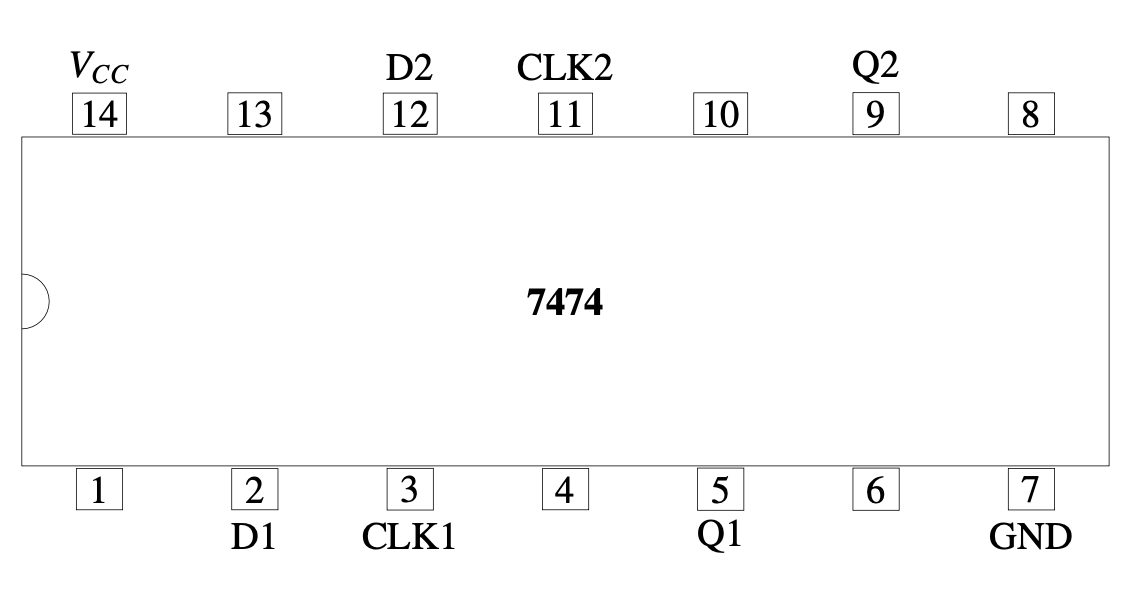
\includegraphics[width=0.45\textwidth]{ic.png} 
 \end{center}\vspace{5mm}
 %----------DFF--------%
  \vspace{2mm}\textbf{D Flip-Flop}
 \begin{center}
 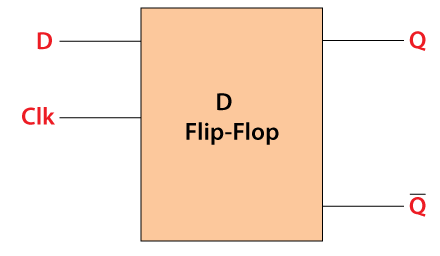
\includegraphics[width=0.45\textwidth]{dff.jpg} 
 \end{center}\vspace{1cm}
 \textbf{Working of D Flip-Flop}

  \setlength{\arrayrulewidth}{0.5mm} \begin{center}
      

  \setlength{\tabcolsep}{25pt}
  \renewcommand{\arraystretch}{1.3}
  \begin{tabular}{|l|c|l|c|}
  \hline 
  \textbf{CLK} & \textbf{D} & \textbf{Q}  & \textbf{$\overline{\textbf{Q}}$}\\
  \hline
    0 & 0 & Q & $\overline{Q}$\\
    0 & 1 & Q & $\overline{Q}$ \\
    1 & 0 & 0 & 1\\
    1 & 1 & 1 & 0\\
    \hline
      \end{tabular}
  \end{center} \vspace{2mm}
  
The D flip-flop is a clocked flip-flop with a single digital input 'D'. \\ Each time a D flip-flop is clocked, its output follows the state of 'D'.\\
\vspace{1cm}
\textbf{Hardware Connections }
\begin{center}
\setlength{\arrayrulewidth}{0.5mm}
\setlength{\tabcolsep}{0.9pt}
\renewcommand{\arraystretch}{2}
    \begin{tabular}{|l|c|l|c|l|c|l|c|l|c|}
    \hline 
    \textbf{Arduino pins} & \textbf{D6} & \textbf{D7} & \textbf{D8} & \textbf{ D9} & \textbf{D2} & \textbf{D3} & \textbf{D4} & \textbf{D5}& \textbf{D13}\\
    \hline
    7474 (2-FF) & 5 & 9 &  &  & 2 & 12 &  &  & CLK \\  \hline
    7474 (1-FF) &  &  & 5 &  &  &  & 2 &  & CLK \\ \hline
    I/P &  &  &   & 5v/GND &  &  &   &    &   \\ \hline
    Detector&  &  &   &  &  &  &   & LED &  \\ 
    \hline
      \end{tabular}
  \end{center}
  
\raggedright  Download the code \\
Github link: \href{https://github.com/chiragshah1244/FWC/blob/main/assignments/assignment_2/code/seq.asm}{Assignment-2}.

\vspace{2mm}\textbf{Command to run the assembly level code }\\
To run : avra file.asm \\

  \end{multicols}
\end{document}